\documentclass[10pt, typeface=serif(roman), pdf,hyperref={unicode}, aspectratio=169]{beamer}
\usepackage{cmap} %поиск pdf
\usepackage[T2A]{fontenc} % кодировка
\usepackage[utf8]{inputenc} % Кодировка исходного текста
\usepackage[english,russian]{babel}  % Локализация и переносы
\usetheme{JuanLesPins}
\usecolortheme{beaver}
\renewcommand{\rmdefault}{cmr}
\usepackage{listings} % для языков программирования


\institute[VFU] % (optional)
{
	«БАЛТИЙСКИЙ ФЕДЕРАЛЬНЫЙ УНИВЕРСИТЕТ ИМЕНИ ИММАНУИЛА КАНТА»
	\and
	Образовательно-научный кластер «Институт высоких технологий»
	\and
	Компьютерная безопасность математические методы защитый информации \\ 3 курс
}
\title{ОТЧЁТ О ЛЕТНЕЙ ПРАКТИКЕ}
\subtitle {Cipher Mode Picker (HKCERT CTF)}
%\author{Нецветайлов Андрей, Флягин Артём}
\author[Arthur, Doe] % (optional, for multiple authors)
{Нецветайлов~А.~А.\and Флягин ~А.~И.}
\date{8 июля 2023}

\usepackage[backend=biber,bibencoding=utf8,sorting=nty,maxcitenames=2,style=numeric-comp]{biblatex}
\addbibresource{library.bib} %для списка литературы

\begin{document}


\frame{\titlepage}



\begin{frame}
	\frametitle{Предисловие}
	Мы выбрали задачу \textbf{Cipher Mode Picker (HKCERT CTF)}. В этой задаче используется криптосистема AES-256. В университете мы её не изучали, нам стало интересно разобраться самим и мы посчитали, что необходимо в рассказать об этом алгоритме в презентации-отчёте; поэтому слайды со 2 до 28 включительно это описание криптосистемы. Решение задачи начинается на 29 слайде.
\end{frame}



\begin{frame}
	\frametitle{Определения}
	\begin{description}
		\item \textbf{Byte} -- целое число от 0 до 255 включительно.
		\item \textbf{Word} -- слово, состоящее из 4 Byte.
		\item \textbf{Nk} -- число 32-битных слов, составляющих шифроключ. Для AES Nk = 4, 6, или 8.
		\item \textbf{Nr} -- число раундов, которое является функцией Nk и Nb. Для AES Nr = 10, 12, 14.
		\item \textbf{Rcon[]} -- массив, который состоит из битов 32-разрядного слова и является постоянным для данного раунда.
		\item \textbf{State} -- промежуточный результат шифрования, который может быть представлен как прямоугольный массив байтов, имеющий 4 строки и Nb колонок.
	\end{description}
\end{frame}
		


\begin{frame}
	\begin{description}
		\frametitle{Определения}
		\item \textbf{Block} -- последовательность бит, из которых состоит input, output, State и Round Key. Также под Block можно понимать последовательность байтов.
		\item \textbf{Cipher Key} -- секретный криптографический ключ, который используется Key Expansion процедурой, чтобы произвести набор ключей для раундов (Round Keys); может быть представлен как прямоугольный массив байтов, имеющий четыре строки и Nk колонок. %расширение ключа
		\item \textbf{Round Key} -- Round Keys получаются из Cipher Key использованием процедуры Key Expansion. Они применяются к State при шифровании и расшифровании.
		\item \textbf{Ciphertext} -- выходные данные алгоритма шифрования.
		\item \textbf{Key Expansion} -- процедура генерации Round Keys из Cipher Key.
	\end{description}

\end{frame}



\begin{frame}
	
	\begin{description}
		\frametitle{Вспомогательные процедуры}
		\item \textbf{AddRoundKey() } -- трансформация при шифровании и обратном шифровании, при которой Round Key XOR’ится c State. Длина RoundKey равна размеру State (то есть если Nb = 4, то длина RoundKey равна 128 бит или 16 байт).
		\item \textbf{InvMixColumns()} -- трансформация при расшифровании, которая является обратной по отношению к MixColumns().
		\item \textbf{InvShiftRows()} -- трансформация при расшифровании, которая является обратной по отношению к ShiftRows().
		\item \textbf{InvSubBytes()} -- трансформация при расшифровании, которая является обратной по отношению к SubBytes().
		\item \textbf{MixColumns()} -- трансформация при шифровании, которая берёт все столбцы State и смешивает их данные (независимо друг от друга), чтобы получить новые столбцы.
	\end{description}
	
\end{frame}
		
		
		
\begin{frame}
	
	\begin{description}
		\item \textbf{RotWord()} -- функция, использующаяся в процедуре Key Expansion, которая берёт 4-байтовое слово и производит над ним циклическую перестановку.
		\item \textbf{ShiftRows()} -- трансформации при шифровании, которые обрабатывают State, циклически смещая последние три строки State на разные величины.
		\frametitle{Вспомогательные процедуры}
		\item \textbf{SubBytes()} -- трансформации при шифровании, которые обрабатывают State, используя нелинейную таблицу замещения байтов (S-box), применяя её независимо к каждому байту State.
		\item \textbf{SubWord()} -- функция, используемая в процедуре Key Expansion, которая берёт на входе четырёхбайтовое слово и, применяя S-box к каждому из четырёх байтов, выдаёт выходное слово.
	\end{description}

\end{frame}



\begin{frame}
	\frametitle{Описание криптосистемы}
	\begin{description}
		\begin{block}
		{
			Определяем размеры Nk и Nr.\\
		}
	\item $ Nk = type/32 $~$ Nr = Nk + 6 $\\
		\end{block}
		\begin{block}
			{
				Генерируем $Nr+1$ раундовый ключ. Каждый раундовый ключ имеет размер 128 бит.\\
			}
		\item $ RoundKey = KeyExpansion(key) $\\
		\end{block}

		\begin{block}
			{
				Смешиваем открытый текст с первым ключом, чтобы лишить возможности аналитика подавать на вход специальный открытый текст\\
			}
		\item $ State = PlainText \oplus RoundKey_1 $\\
		\end{block}
	\end{description}
\end{frame}



\begin{frame}
	\frametitle{Описание криптосистемы}
	\begin{description}
		\begin{block}
			{
				Для \textit{i = 1,...,Nr-1} - выполняем
			}
			\item $ State = Raund(State, RaundKey_{i+1}) $\\
		\end{block}
		\begin{block}
			{
				Последний раунд отличается от остальных
			}
			\item $ State = EndRaund(State, RaundKey_{Nr+1}) $\\
		\end{block}
		\begin{block}
			{
				Вывод результата
			}
			\item $ CipherText = State $\\
		\end{block}
	\end{description}
\end{frame}



\begin{frame}
	\frametitle{Описание Round}
	\begin{description}
		\begin{block}
			{
				Input
			}
			\item $ State= (s_1,...,s_16), s_i - Byte $ \\
			$ RoundKey = (k_1,...,k_16), k_i - Byte$\\
		\end{block}
		\begin{block}
			{
				Output
			}
			\item $ State= (s_1,...,s_16), s_i - Byte $\\
		\end{block}
	\end{description}
	\begin{enumerate}
		\item $State = SubBytes(State)$
		\item $State = ShiftRows (State)$
		\item $State = MixColumns(State)$
		\item State = $State \oplus RoundKey$
	\end{enumerate}
\end{frame}



\begin{frame}
	\frametitle{Описание EndRound}
	\begin{description}
		\begin{block}
			{
				Input
			}
			\item $ State= (s_1,...,s_16), s_i - Byte $ \\
			$ RoundKey = (k_1,...,k_16), k_i - Byte$\\
		\end{block}
		\begin{block}
			{
				Output
			}
			\item $ State= (s_1,...,s_16), s_i - Byte $\\
		\end{block}
	\end{description}
	\begin{enumerate}
		\item $State = SubBytes(State)$
		\item $State = ShiftRows (State)$
		\item $State = State \oplus RoundKey $
	\end{enumerate}
\end{frame}



\begin{frame}
	\frametitle{Описание SubBytes()}
	Процедура SubBytes() обрабатывает каждый байт состояния, независимо производя нелинейную замену байтов, используя таблицу замен (S-box). Такая операция обеспечивает нелинейность алгоритма шифрования.
	\begin{enumerate}
		\begin{block}
			{
				Построение S-box
			}
			\item Взятие обратного числа в $ GF(2^8) $\\
			\item К каждому байту, принадлежащему S-box, применяется операция:
			\begin{description}
				\item $ b'_i = b_i \oplus b_{i+4 mod 8} \oplus b_{i+5 mod 8 } \oplus b_{i+7 mod 8} \oplus c_i $
				\item где $ 0 \leq i < 8 $, и где $ b_i $ есть $i$-ый бит константы $ c = 63  16 = 99 10 = 01100011_2  $
			\end{description}
		\end{block}
		\begin{figure}
			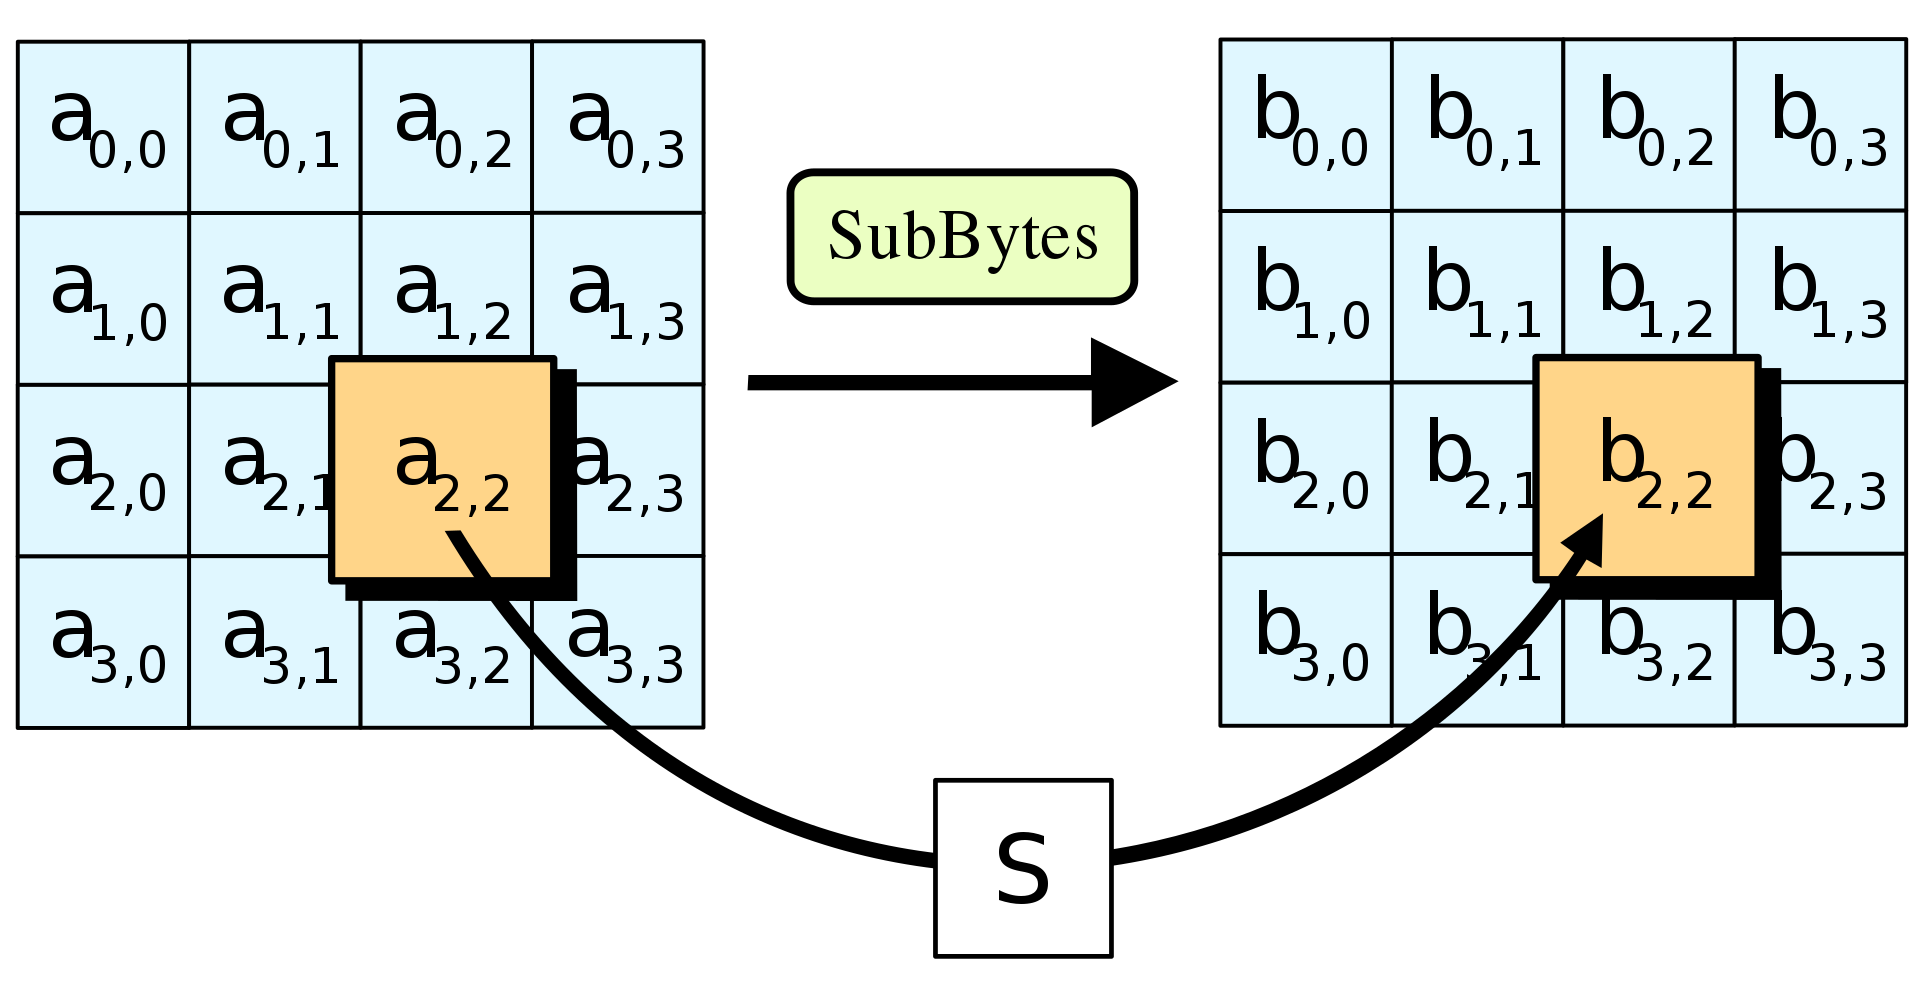
\includegraphics[scale=0.075]{S-box.png}	
		\end{figure}
	\end{enumerate}
\end{frame}



\begin{frame}
	\frametitle{Немного математики}
	\begin{block}
		{
			Операция сложения в \(GF(2^8)\)
		}
		\begin{description}
			\item \[ GF(2^8) = \{s_7,s_6,s_5,s_4,s_3,s_2,s_1,s_0\}, ~s_i \in \mathbb{Z}_2\]
			\item Элемент \[ (s_7,s_6,...,s_0) = s_72^7 + s_62^6 + ... + s_12 + s_0 \] назовём \textbf{байтом }
			\item Отождествим каждый байт с многочленом \[ (s_7,...,s_1,s_0) \leftrightarrow s_7x^7 + ... + s_1x + s_0 \]
		\end{description}
	\end{block}
	Из вышесказанного, сумму байт можно отождествить с побитовой операцией XOR.
\end{frame}



\begin{frame}
	\frametitle{Немного математики}
	\begin{block}
		{
			Операция умножения в \(GF(2^8)\)
		}
		\begin{description}
			\item Определим операцию умножения при помощи многочлена \[x^8+x^4+x^3+x+1\]
			\item \(\exists s(x)\) и \(t(x)\) - многочлены 7 степени в \(GF(2^8)\)
			\item Разделим их произведение на \(f(x)\): \[s(x)t(x)=g(x)f(x)+r(x), ~deg(f(x)) < 8\]
			тогда \[s(x)*t(x)=r(x)\]
		\end{description}
	\end{block}
\end{frame}



\begin{frame}
	\frametitle{Немного математики}
	\begin{block}
		{
			Операция умножения в \(GF(2^8)\)
		}
		\begin{description}
			\item По расширенному алгоритму Евклида: \[u(x)s(x)+v(x)f(x)= \gcd (s(x),f(x))\]
			\item Если \[\gcd (s(x),f(x)) = 1\] то \[(u(x))^{-1} = s(x)\]  иначе \(s(x)\) необратим
		\end{description}
	\end{block}
	Если gcd равен 1 \(\Rightarrow ~f(x)\) раскладывается на множители над \(\mathbb{Z}_2(\). Но \(f(x)\) неприводим по условию. Из всего вышеперечисленного следует, что \(GF(2^8)\) - поле.
\end{frame}



\begin{frame}
	\frametitle{Матрица S-box}
	Байт \textit{y} будет заменять байт \textit{x} по правилу:
	\[y = Ax^{-1}+b\] где\\
	\(x^{-1}\) - обратный в \(GF(2^8)\)
\end{frame}



\begin{frame}
	\frametitle{Шифр перестановки ShiftRows}
	\[State =
	\begin{bmatrix}
		s_1 & s^5 & s^9 & s^{13} \\
		s^2 & s^6 & s^{10} & s^{14} \\
		s^3 & s^7 & s^{11} & s^{15} \\
		s^4 & s^8 & s^{12} & s^{16} \\
	\end{bmatrix}\]
	Второй, третий и четвёртый ряд сдвигаются влево на 1, 2, 3 соответственно:
	\[State =
	\begin{bmatrix}
		s_1 & s^5 & s^9 & s^{13} \\
		s^2 & s^6 & s^{10} & s^{14} \\
		s^3 & s^7 & s^{11} & s^{15} \\
		s^4 & s^8 & s^{12} & s^{16} \\
	\end{bmatrix}
	\rightarrow
	\begin{bmatrix}
		s_1 & s^5 & s^9 & s^{13} \\
		s^6 & s^{10} & s^{14} & s^2\\
		s^{11} & s^{15} & s^3 & s^7\\
		s^{16} & s^4 & s^8 & s^{12}\\
	\end{bmatrix}\]
\end{frame}




\begin{frame}
	\frametitle{Ещё немного математики}
	Расширим \(GF(2^8)\), присоединив многочлен \(x^4+1\)
	Зададим множество \(s_1,s_2,s_3,s_4\), ~~\(s_i \in GF(2^8)\)
	\begin{block}
		{
			Сложение в \( GF(2^8)_{x^4+1}\)
		}
		\[ (s_1,s_2,s_3,s_4) + (t_1,t_2,t_3,t_4) = (s_1+t_1,s_2+t_2,s_3+t_3,s_4+t_4)\] \\
		\[\forall s_i+t_i \in GF(2^8)\]
	\end{block}
	\begin{block}
		{
			Умножение в \( GF(2^8)_{x^4+1}\)
		}
		\[ s(x) = s_1+s_2x+s_3x^2+s_4x^3\] \\
		\[s(x) \times t(x) = s(x)t(x) (mod x^4+1) = k(x)\]
		\[s(x),t(x),k(x) \in GF(2^8)\]
	\end{block}
\end{frame}



\begin{frame}
	\frametitle{Ещё немного математики}
	\begin{block}
		{
			Делители нуля в \(GF(2^8)_{x^4+1}\)\\
			\(\sphericalangle ~x^4+1\) 
		}
		\[x^4+1 = (x-1)^4 \Rightarrow (x^2 + 1)(x^2+1) = 0 ~(mod x^4+1)\]
		Таким образом, в \( GF(2^8)_{x^4+1}\) существуют делители нуля и \( GF(2^8)_{x^4+1}\) -- кольцо.
	\end{block}
\end{frame}



\begin{frame}
	\frametitle{Ещё немного математики}
	\begin{block}
		{
			Более подробно об умножение в \( GF(2^8)_{x^4+1}\)
		}
		При делении с остатком на \(x^4+1\) можно считать, что \(x^4 + 1 = 0\) или \\
		\(x^4=-1=1\), тогда:
		\(a_1+a_2x+a_3x^2+a_4x^3)(s_1+s_2x+s_3x^2+s_4x^3)=a_1s_1+(a_2s_1+a_1s_2)x+(a_3s_1+a_2s_2+a_1s_3)x^2+(+a_4s_1+a_3s_2+a_2s_3+a-1s_4)x^3+(a_4s_2+a_3s_3+a_2s_4)x^4+(a_4s_3+a_3+s_4)x^5+a_4s_4x^6 = a_1s_1+a_4s_2+a_3s_3+a_2s_4+(s_1+s_2x+s_3x^2+s_4x^3)x+(a_3s_1+a_2s_2+a_1s_3+a_4s_4)x^2+(+a_4s_1+a_3s_2+a_2s_3+a_1s_4)x^3\)
	\end{block}
	\[as =
	\begin{bmatrix}
		a_1 & a^4 & a^3 & a^2 \\
		a^2 & a^1 & a^4 & a^3 \\
		s^3 & a^2 & a^1 & a^4 \\
		s^4 & a^3 & a^2 & a^1 \\
	\end{bmatrix}
	\begin{bmatrix}
		s_1 \\ s_2 \\ s_3 \\s_4
	\end{bmatrix}\]
\end{frame}



\begin{frame}
	\frametitle{MixColumns}
	\begin{block}
		{
			Функция перемножает State и многочлен \(a(x)\) в \(GF(2^8)_{x^4+1}\)
		}
		\[State =
		\begin{bmatrix}
			s_1 & s^5 & s^9 & s^{13} \\
			s^2 & s^6 & s^{10} & s^{14} \\
			s^3 & s^7 & s^{11} & s^{15} \\
			s^4 & s^8 & s^{12} & s^{16} \\
		\end{bmatrix}\]
		\[a(x) = 2+x+x^2+3x^3\]
		
	\end{block}
\end{frame}



\begin{frame}
	\frametitle{Cipher Key}
	\begin{block}
		{
			Input
		}
		Nk -- количество слов в ключе \textit{key}.
		Nr -- количество раундов в алгоритме.
		\[key = (k_1,k_2,...,k_{4Nk})\]
		\(k_i\) -- байт
		
	\end{block}
	\begin{block}
		{
			Output
		}
		Расширенный ключ
		\[w = (w_0,w_1,...,w_{4Nr+1}-1)\]
		\[RoundKey_i = (w_{4i-4},w_{ri-3},w_{4i-2},w_{4i-1})\]
	\end{block}
\end{frame}



\begin{frame}
	\frametitle{Cipher Key}
	\begin{enumerate}
		\item Для \(i = 0,..,Nk-1:\)\\
		~~~~\(w_i = (k_{4i+1},k_{4i+2},k_{4i+3},k_{4i+4})\)
		\item Для \(i=Nk,...,4(Nk+1)-1:\)\\
		~~~~\(temp = w_{i-1}\)\\
		~~~~Если \(i \equiv 0 (mod ~Nk)\)\\
		~~~~~~~~то: \(temp = SubWord(RotWord(temp)) \oplus Rcon(i/Nk)\) \\
		~~~~~~~~иначе:\\
		~~~~~~~~~~~~Если \(Nk > 6 and i \equiv 4 (mod~Nk)\)\\
		~~~~~~~~~~~~то: \(temp = SubWord(temp)\)\\
		~~~~\(w_i = temp \oplus w_{i-Nk}\)
		\item Output (Nr+1 сеансовых ключа):\\
		\((w_0,w_1,w_2,w_3),...,(w_{4Nk},w_{4Nk+1},w_{4Nk+2},w_{4Nk+3})\)
	\end{enumerate}
	
\end{frame}

\begin{frame}
	\frametitle{Вспомогательные функции}
	\begin{block}
		{
			SubWord()
		}
		\(SubWord(w) = Subword((w_1,w_2,w_3,w_4)) = (SubBytes(w_1),SubBytes(w_2),SubBytes(w_3),SubBytes(w_4))\)\\ \(w_i\) - байт.
	\end{block}
	\begin{block}
		{
			RotWord()
		}
		\(RotWord(w) = RotateLeft(w,1)\)
	\end{block}
	\begin{block}
		{
			Rcon()
		}
		\(Rcon(i) = (2^{i-1},0,0,0)\)\\
		\(2^{i-1}\) -- возведение в степень в \(GF(2^8)\)
	\end{block}
\end{frame}



\begin{frame}
	\frametitle{Заполнение сообщения}
	\begin{block}
		{
			Необходимые требования
		}
		\begin{itemize}
			\item Сообщение должно быть определённой длины
			\item Чтобы шифровать сообщение произвольной длины, необходим алгоритм дополнения входных данных до нужной длины
			\item У этого алгоритма должен быть обратный алгоритм, который может восстановить сообщение по дополненной части.
		\end{itemize}
	\end{block}
\end{frame}



\begin{frame}
	\frametitle{Заполнение сообщения}
	\begin{block}
		{
			Input
		}
		\(m = (m_1,m_2,...,m_k, ~m_i)\) -- байт
	\end{block}
	\begin{block}
		{
			Output
		}
		\(M = (M_1,M_2,...,M_L), ~M_{i}\) -- блок\\
		\(M_i = (M_{i,1},...,M_{i,16}), ~M_{i,j}\) -- байт
	\end{block}
	\begin{enumerate}
		\item Вычисляем количество недостающих байт
		\[n = 16 - Mod(k,16)\]
		\item К \(m\) справа добавляем \(n\) байт, равных n.
		\item Разбиваем сообщение \(m\) на блоки по 16 байт.
	\end{enumerate}
\end{frame}



\begin{frame}
	\frametitle{Режим шифрования}
	\textbf{Режим шифрования} -- метод применения блочного шифра (алгоритма), позволяющий преобразовать последовательность блоков открытых данных в последовательность блоков зашифрованных данных. При этом для шифрования одного блока могут использоваться данные другого блока.\\
	Обычно режимы шифрования используются для изменения процесса шифрования так, чтобы результат шифрования каждого блока был уникальным вне зависимости от шифруемых данных и не позволял сделать какие-либо выводы об их структуре. Это обусловлено, прежде всего, тем, что блочные шифры шифруют данные блоками фиксированного размера, и поэтому существует потенциальная возможность утечки информации о повторяющихся частях данных, шифруемых на одном и том же ключе. \\
	Для решения задачи используются CFB и OFB, поэтому мы рассмотрим только их.
\end{frame}



\begin{frame}
	\frametitle{Cipher Feedback}
	\begin{block}
		{
			 Во время шифрования каждый блок открытого текста складывается по модулю 2 с блоком, зашифрованным на предыдущем шаге. 
		}
		~~\(C_0 = IV\)\\
		~~\(C_i = E_k(C_{i-1},k \oplus P_i )\)\\
		~~\(P_i = E_k(C_{i-1},k \oplus C_i )\)\\
	\end{block}
	\begin{figure}
		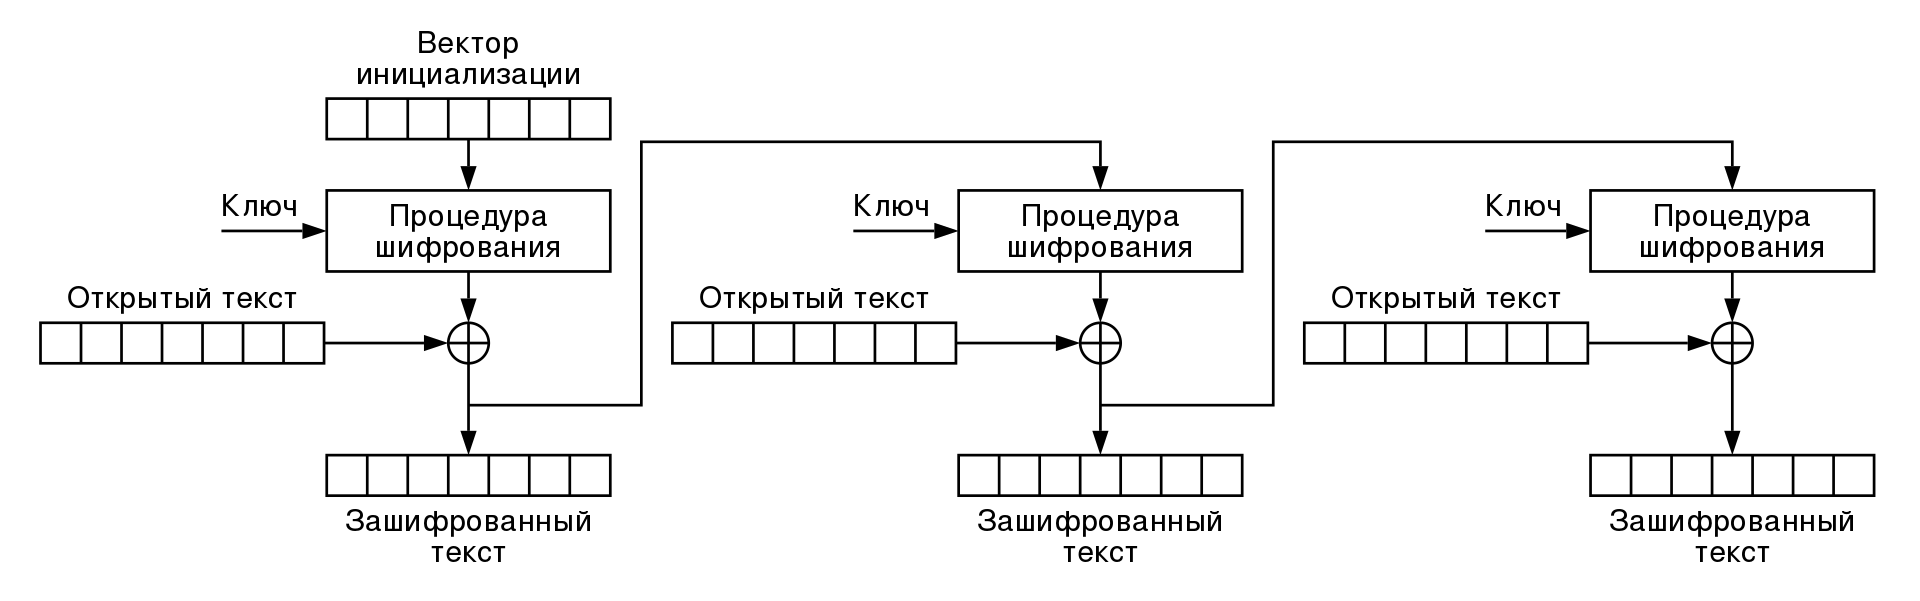
\includegraphics[scale=0.18]{Шифрование в режиме обратной связи по шифротексту.png}	
	\end{figure}
\end{frame}



\begin{frame}
	\frametitle{Output Feedback}
	\begin{block}
		{
			Режим (OFB) обратной связи вывода превращает блочный шифр в синхронный шифр потока: он генерирует ключевые блоки, которые являются результатом сложения с блоками открытого текста, чтобы получить зашифрованный текст. Так же, как с другими шифрами потока, зеркальное отражение в зашифрованном тексте производит зеркально отражённый бит в открытом тексте в том же самом местоположении. Это свойство позволяет многим кодам с исправлением ошибок функционировать как обычно, даже когда исправление ошибок применено перед кодированием.\\		
			Из-за симметрии операции сложения, шифрование и расшифрование похожи: 
		}
		~~\(C_i = P_i \oplus O_i )\)\\
		~~\(P_i = C_i \oplus O_i )\)\\
		~~\(O_i = E_k (O_{i-1})\)\\
		~~\(C_0 = IV\)\\
	\end{block}
\end{frame}


\begin{frame}
	\frametitle{Output Feedback}
	\begin{block}
		{
			Шифрование в режиме OFB
		}
		\begin{figure}
			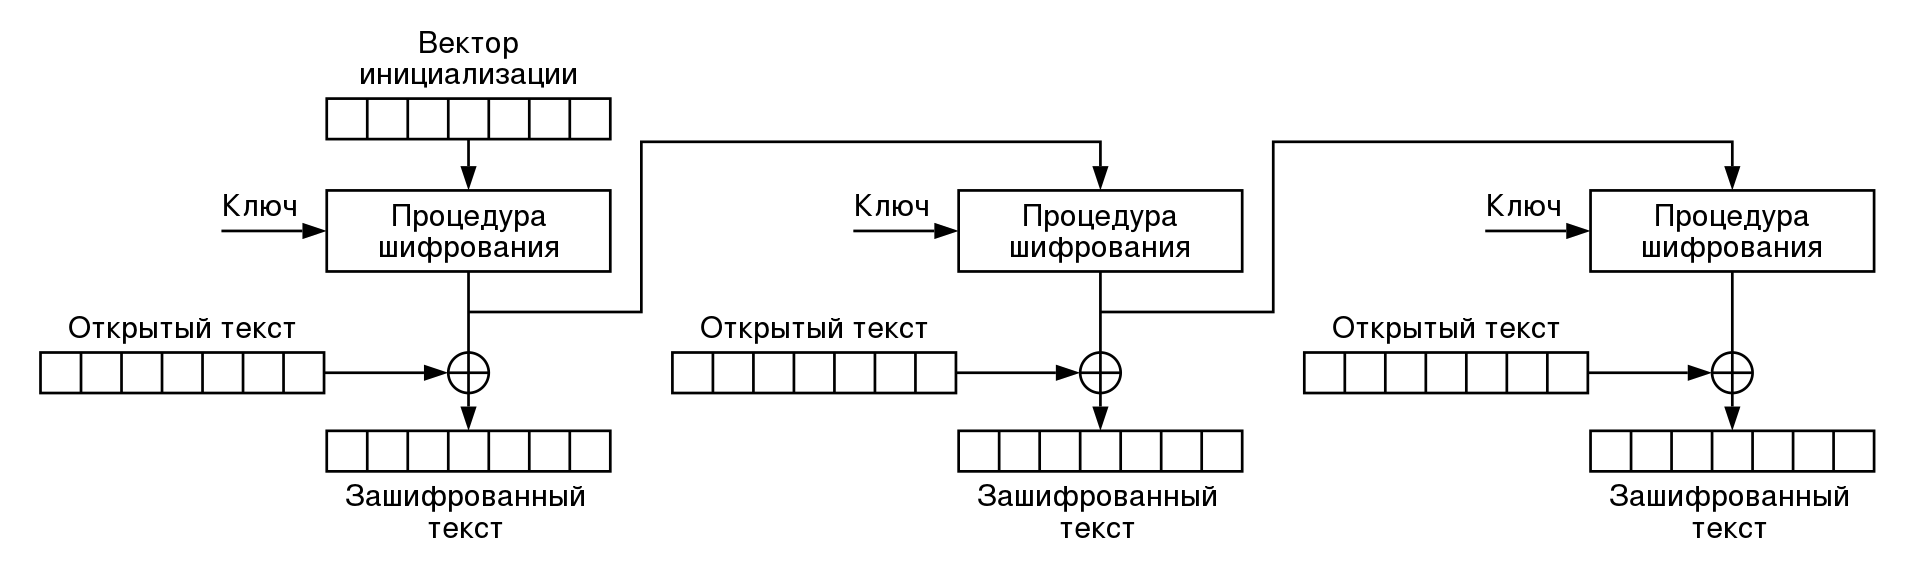
\includegraphics[scale=0.14]{Шифрование в режиме OFB.png}	
		\end{figure}
	\end{block}
	\begin{block}
		{
			Расшифрование в режиме OFB
		}
		\begin{figure}
			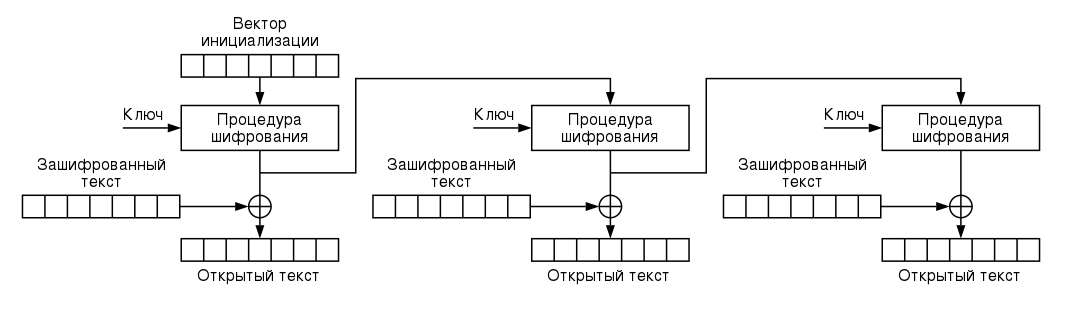
\includegraphics[scale=0.22]{Расшифрование в режиме OFB.png}	
		\end{figure}
	\end{block}
\end{frame}



\begin{frame}
	\frametitle{Решение}
	\begin{block}
		{
			Из приложенного файла можно сделать следующие выводы
		}
		\begin{enumerate}
			\item Длина флага 80 символов.
			\item \(key\) и \(IV\) используются для каждого соединения.
			\item Реализовано пять режимов шифрования: 'ECB', 'CBC', 'CFB', 'OFB', 'CTR'
		\end{enumerate}
	\end{block}
	Мы можем дать серверу данные для шифрования, позволить серверу шифровать флаг в течении 5 минут за одно подключение. Но можем использовать только один режим шифрования за одно подключение.
	Выше мы рассмотрели функции CFB и OFB. Они практически идентичны, поэтому мы их и будем использовать
\end{frame}



\begin{frame}
	\frametitle{Решение}
	Введём на вход нули и применим CFB, он вернёт шифрование каждого блока. Затем запросим зашифрованный флаг с режимом OFB. Объедем их вместе и получим флаг.
	\begin{block}
		{
			Код для CFB
		}
		\(C_0 = IV\)\\
		\(C_i = E_k(C_{i-1}) \oplus P_i\)\\
		\(P = 0 \Rightarrow C_i = E_k(C_{i-1})\)\\
	\end{block}
	\begin{block}
		{
			Код для OFB
		}
		\(O_0 = IV\)\\
		\(O_i = E_k(O_{i-1})\)\\
		\(C_i = E_k(O_{i-1}) \oplus P_i\)
	\end{block}
\end{frame}



\begin{frame}
	\frametitle{Код программы}
	\lstinputlisting[language=Python]{solution.py}
\end{frame}



\begin{frame}
	\frametitle{Ответ}
	\begin{block}
		{Флаг}
		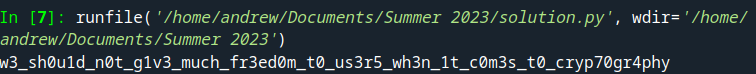
\includegraphics[scale=0.935]{flag.png}
	\end{block}
	\begin{block}
		{Ответ}
		hkcert21\{w3\_sh0u1d\_n0t\_g1v3\_much\_fr3ed0m\_t0\_us3r5\_wh3n\_1t\_c0m3s\_t0\_cryp70gr4phy\}
	\end{block}
	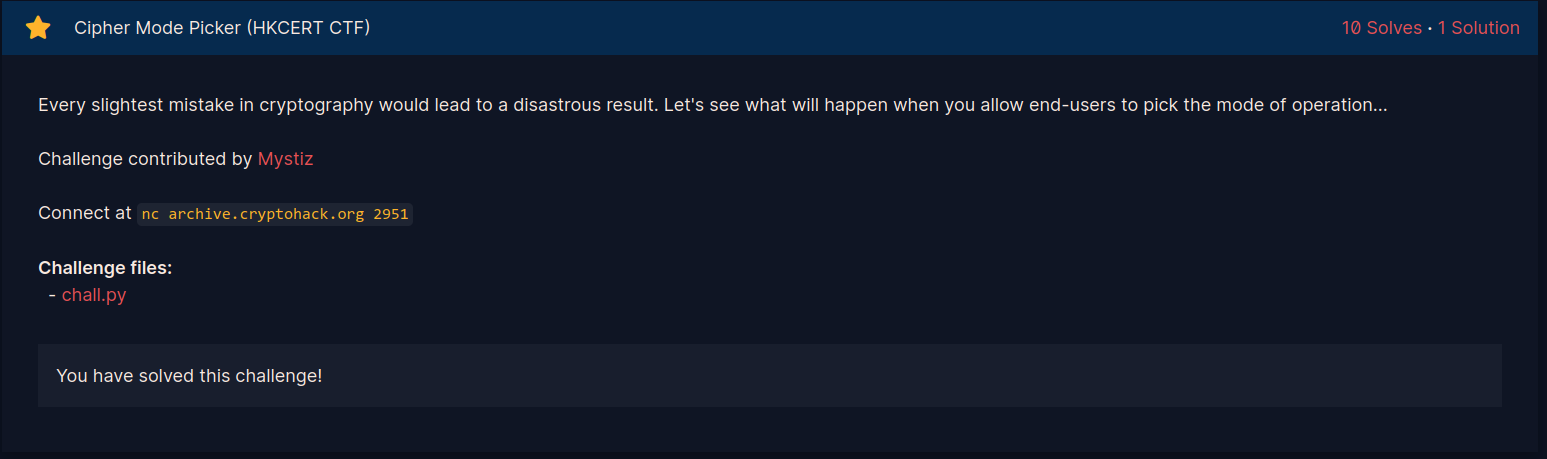
\includegraphics[scale=0.45]{Решено.png}
\end{frame}



\end{document}